%% \section{Theoretical Foundations: Mathematical Models and Algorithms for Radar-Based Object Detection}
%% \label{sec:Mathematical Models and Algorithms for Radar-Based Object Detection}

\section{Pipeline implementation: Modules implemented and mathematical explanation}
\label{sec:Mathematical Models and Algorithms for Radar-Based Object Detection}
As the radar sensor outputs its raw data in frames which contain a raw point cloud, a modular processing pipeline was developed.
This pipeline consists of different modules implementing the needed stages for pre-processing the sensor's data, filtering the point cloud, clustering and object detection.
The modular design allows the modification and adaption to different environments.
\par
In a pre-processing stage, the sensor's raw data frames, obtained via UART, are decoded and translated into frames containing individual points in a usable format with information about their $x,y,z,v_{r}$ and $SNR$ values.
They are then passed into a "Frame Aggregator" which stores a certain amount of frames in order to supply the later stages with the data from multiple frames and thus compensate for possible data sparsity.
The aggregated data is filtered by multiple filtering stages, starting with static parameters for the spatial dimension and the SNR, followed by a dynamic filtering stage using a comparison of the vehicle's estimated self-speed to the points' speeds for filtering.
The filtered points are then clustered using a two-stage approach and forwarded to the brake controller for object detection. The reason for the 2 stages of clustering is that for any given object that may be detected there would be noise or segmentation caused by some space between objects. So this 2 stages help us discard information that could be just a reflection and focus into the points that are considered as objects. This being done by having a permissive first stage, and afterwards a strict clustering stage to be able to label an object with a cluster ID for further processing.
\begin{figure}[!htbp]
    \centering
    \resizebox{0.48\textwidth}{!}{
        \begin{tikzpicture}
            % Block styles
            \tikzstyle{block} = [rectangle, draw, text width=4.5em, text centered, minimum width=6em, minimum height=4em]
            \tikzstyle{block_dashed} = [rectangle, draw, text width=2em, text centered, minimum width=4em, minimum height=4em, dashed]
            % Input and output
            \node[block] (uart) {UART\\Data};
            \node[block, right=of uart] (decoder) {Data decoder};
            \node[block, right=of decoder] (frames) {Frame};
            \node[block, right=of frames] (frame_aggr) {Frame\\Aggregator};
            \node[block, right=of frame_aggr] (coord_filter) {Filter\\$x,y,z$\\$\phi,SNR$};
            \node[block, right=of coord_filter] (self_speed_estim) {Self-speed Estimator};
            \node[block, right=of self_speed_estim] (self_speed_kalman) {Kalman Filter};
            \node[block, below=of self_speed_estim] (ve_speed_calc) {Calculation\\of $v_{e}$};
            \node[block, right=of ve_speed_calc] (ve_filter) {Filter\\$v_{e}$ vs. self-speed};
            \node[block, right=of ve_filter] (clustering) {Clustering};
            \node[block, right=of clustering] (brake_controller) {Brake\\Controller};
            % Connections
            \draw[->] (uart) -- (decoder);
            \draw[->] (decoder) -- (frames);
            \draw[->] (frames) -- (frame_aggr); % Connection from antenna to RF amplifier
            \draw[->] (frame_aggr) -- (coord_filter);
            \draw[->] (coord_filter) -- (self_speed_estim);
            \draw[->] (coord_filter.south) |- (ve_speed_calc.west);
            \draw[->] (self_speed_estim) -- (self_speed_kalman);
            \draw[->] (self_speed_kalman) -- (ve_filter);
            \draw[->] (ve_speed_calc) -- (ve_filter);
            \draw[->] (ve_filter) -- (clustering);
            \draw[->] (clustering) -- (brake_controller);

            \draw [decorate, decoration = {brace, mirror, raise=10pt}] (uart.south west) --  (frames.south east) node[pos=0.5,below=15pt,black]{Sensor Data Preprocessing};
        \end{tikzpicture}
    }
    \caption{Block diagram of the pipeline}
    \label{fig:block_diag_pipeline}
\end{figure}

\FloatBarrier\noindent

%\begin{figure}[!htbp]
%    \centering
%    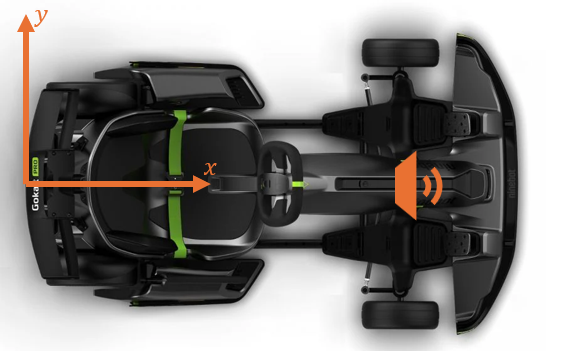
\includegraphics[width=1.0\linewidth]{images/ninebot.png}
%    \caption{Schematic sensor distribution}
%    \label{fig: One sensor is located in the front of the test vehicle}
%\end{figure}
%\FloatBarrier\noindent